\lhead{\emph{Capitolo 1}}
\chapter{Stato dell'arte} 
L'obiettivo di questo capitolo introduttivo e quello di mostrare quali sono gli approcci esistenti per lo sviluppo di applicazioni su dispositivi mobili ed analizzarne i vantaggi e gli svantaggi.
In particolare per lo sviluppo di applicazioni multi piattaforma si introdurranno una serie di tecnologie che tutt'oggi possono essere utilizzate per la creazione di applicazioni ibride.

\section{Sviluppo Nativo}
Dopo un'attenta analisi dei requisiti, una delle strade percorribili quando si intende sviluppare un'applicazione mobile è quella di orientarsi verso lo sviluppo nativo, ovvero utilizzare il linguaggio di programmazione specifico per una determinata piattaforma.

Lo sviluppo nativo implica competenze specifiche e capacità di sviluppo sui più diffusi sistemi operativi: iOS, Android, Windows Phone, la tabella seguente \ref{tbl: TabellaOS} indica i linguaggi utilizzati nelle rispettive piattaforme:

\begin{table}[h]
	\centering
    	\begin{tabular}{cc}
      	\hline
        	\textbf{Sistema Operativo} & \textbf{Linguaggi/o}     \\ \hline
        	iOS                        & ObjectiveC / Swift       \\ \hline
        	Android                    & Java                     \\ \hline
        	Windows Phone              & .NET                     \\ \hline
        	BlackBerry                 & C++ / Qt                 \\ \hline
        	FirefoxOS                  & Javascript + CSS + HTML5 \\ \hline
    	\end{tabular}
    	\caption{Lista dei vari linguaggi di programmazione utilizzati nei sistemi operativi per dispositivi 		
    			 mobili}
		\label{tbl: TabellaOS}
\end{table}

Dato l'obiettivo prefissatosi nell'introduzione di avere la stessa applicazione disponibile su più piattaforme, con questo tipo di approccio la soluzione si risolve semplicemente sviluppando la stessa applicazione più volte per ogni piattaforma che si è scelto. 
Molto banalmente se un ipotetico cliente chiedesse di avere la sua applicazione disponibile su Windows Phone, Android e iOS lo sviluppatore dovrà creare rispettivamente 3 applicazioni distinte in .Net, Java e ObjectiveC ovviamente senza la possibilità di riutilizzare il codice tra un linguaggio e l'altro.

Come si può notare, se si  vuole usare questo tipo di approccio con l'idea di avere una applicazione su più piattaforme lo svantaggio più grande è sicuramente quello dei tempi e dei costi di sviluppo, ipoteticamente si potrebbe disporre di più programmatori con competenze specifiche nei vari linguaggi, ma questo sicuramente ridurrebbe la competitività del prezzo dell'applicazione al cliente. Inoltre per i programmatori anche sviluppare in diversi linguaggi la stessa applicazione comporta a usare modelli di progettazione differenti e quindi una re-ingegnerizzazione dell'applicazione per ogni piattaforma.
Alcuni dei vantaggi di questo approccio sono:

\begin{itemize}
\item Massima performance in termini di potenza di calcolo e di sfruttamento del processore.
\item Si ha il pieno controllo dei sensori del dispositivo
\item Si sfruttano tutte le caratteristiche specifiche della piattaforma, sia in termini di software (librerie del produttore o di terze parti) che di hardware (del dispositivo o esterno)
\end{itemize}

Si ha quindi a discapito dei costi e dei tempi produzione una buona resa dell'applicazione a livello di prestazioni e di utilizzo completo delle caratteristiche del dispositivo. Questo tipo di approccio infatti è molto conveniente quando l'applicazione richiede un utilizzo molto intenso e performante delle risorse.

Prima di evidenziare quali sono i vantaggi e gli svantaggi differenti tra i vari approcci, si vedrà che cosa comporta effettivamente usare altri modelli di sviluppo e di quali tecnologie è richiesta la conoscenza per valutarne alla fine i costi nei vari termini.  

\section{Mobile Web Applications}

Con l'evolversi delle tecnologie web si ha abbandonato sempre di più il concetto di \emph{Sito Web} o \emph{Sito Internet} e introdotto il termine \emph{Applicazione Web}. Questo fatto è dovuto al continuo potenziamento dei linguaggi e degli strumenti che si utilizzano in ambito web, basta prendere come esempio Javascript, i primi standard di ECMAscript avevano solo il ruolo di dare animazione alla pagina HTML e di interfacciarsi con Applet Java, oggi si possono trovare Framework Javascript per ogni tipo di esigenza come per esempio: gestione dei contenuti di una pagina web, generatori di documentazione, test di codice, grafica 3D ecc\ldots. Inoltre si può riscontrare l'evoluzione dell'HTML verso un linguaggio sempre più ricco di funzionalità grazie al quale si può definire ora interfacce utente interattive con la possibilità di un design accattivante grazie ai fogli si stile(CSS3). Ma il vero motivo per cui oggi si parla di  \emph{Web Applications} è dato dall'utilizzo che si fa delle tecnologie Web e dello scopo che si da alle applicazioni, come ad esempio l'esecuzione di programmi direttamente sul browser web che rimandano la computazione ad un server senza preoccuparsi di installare il programma sul proprio computer.

Un importante passo che ha favorito l’evolversi dei Siti Web in Applicazione Web, e ad essere fruito tramite dispositivi mobili, è stato il concetto di \emph{Responsive Web Application}. Si potrebbe tradurre in italiano la parola \emph{Responsive} come \emph{Adattato/a}, che sostanzialmente si tratta in una ri-organizzazione dei contenuti della pagina. Il fattore che influisce su questo comportamento è la dimensione dello schermo del dispositivo, essendo gli smartphone, tablet di dimensioni ridotte rispetto allo schermo di un computer, quello che fa una \emph{Responsive Web Application} è adattare i propri contenuti alla dimensione dello schermo del dispositivo, il tutto in modo completamente automatico, senza il bisogno dell'utente di ingrandire con le dita i contenuti. Si potrebbe pensare a primo impatto che si tratti soltanto di una riduzione delle dimensioni della pagina web, in realtà entra in gioco un meccanismo che cambia le proporzioni e la disposizione dei contenuti rendendo ben visibile e nitido il testo e le immagini.
   
Da quanto appena detto, possiamo constatare che l'obiettivo di avere una Applicazione multi piattaforma che ci siamo prefissati all'inizio della tesi è molto comodo sotto questo tipo di approccio. Al contrario dello sviluppo nativo, non dobbiamo preoccuparci di dover programmare la stessa applicazione per diversi sistemi operativi in quanto il codice che scriviamo viene interpretato dal browser web il quale non dipende dalla piattaforma dalla quale stiamo utilizzando l'applicazione.

Le conoscenze che sono richieste al programmatore per poter affrontare un approccio di questo genere sono sicuramente quelle dei linguaggi HTML, CSS e Javascript, pacchetto di competenze che ritroviamo in tutti i programmatori che generalmente si occupano dello sviluppo di siti web. Ne deduciamo che rispetto all'approccio nativo abbiamo un costo sicuramente molto inferiore in termini di conoscenze e di tempi di sviluppo per un risultato ottimale rispetto agli obiettivi prefissati, ma ci sono dei fattori negativi in questo tipo di approccio decisamente non trascurabili.

Come i siti web anche le applicazioni web necessitano di una connessione ad Internet sempre presente per per funzionare, e di conseguenza se il dispositivo che si sta utilizzando è offline queste applicazioni non possono essere raggiunte / utilizzate, parametro che è sicuramente rilevante nella scelta di applicazioni da parte dell'utente. Quello che un fruitore si aspetta di trovare in una applicazione è che sia sempre reperibile anche se la connessione ad Internet in quel momento non è presente. Inoltre dal browser le	 Web Application non possono accedere direttamente alle funzionalità del dispositivo e usufruire ad esempio della fotocamera, il gps o la gestione delle risorse del dispositivo. Altra nota negativa delle applicazioni web riguarda il salvataggio dei dati che risulta molto difficile non potendo accedere alla memoria del dispositivo, tramite browser si potrebbero memorizzare alcuni dati in cache ma correrebbero il rischio di venire cancellati ad insaputa dell'utente, l'unica soluzione è accedere ai dati una volta connessi ad internet tramite un processo di accounting fornito dall'applicazione, il problema è che ogni utente dovrebbe avere diversi account per ogni applicazione che utilizza, cosa non sempre molto gradita dall'utente.

\section{Confronto tra i due approcci}

Nelle descrizioni precedenti si è visto che tra i due approcci utilizzati il rapporto che caratterizza il confronto del tipo di sviluppo è tra Prestazioni e User Experience ottimale nello sviluppo nativo / bassi costi di produzione e velocità di sviluppo tramite Web Application. Quando si sviluppano applicazioni Mobile in generale bisogna tenere conto di diversi fattori di valutazione che riguardano principalmente l'utente finale ma con un occhio ache agli sviluppatori, ecco quindi come si comportano gli approcci precedentemente visti su una serie di fattori che ho ritenuto più rilevanti di altri:

\begin{description}

\item[Immediatezza]Le web application sono immediatamente disponibili agli utenti tramite un browser su una gamma di dispositivi (iPhone, Android, BlackBerry, ecc.). Le applicazioni mobile native invece richiedono che l'utente innanzitutto scarichi e installi l'applicazione da un mercato prima che il contenuto o l'applicazione possa essere utilizzata.
\item[Compatibilità] un unico sito web mobile può raggiungere gli utenti attraverso diversi tipi di dispositivi mobili, mentre applicazioni native richiedono una versione separata da sviluppare per ogni tipo di dispositivo. Inoltre, le URL delle web app mobile sono facilmente integrabili all'interno di altre tecnologie mobile come gli SMS, i codici QR e NFC.
\item[Capacità di aggiornamento] una web app è molto più dinamica di un'applicazione mobile in termini di flessibilità pura per aggiornare il contenuto. Se si desidera modificare la struttura o il contenuto di una web app mobile è sufficiente pubblicare la modifica una volta e le modifiche sono immediatamente visibili; l'aggiornamento di un app, dall'altro richiede gli aggiornamenti siano convogliati agli utenti, che poi devono essere scaricati in modo da aggiornare l'applicazione su ogni tipo di dispositivo.
\item[Ricercabilità] le web app sono maggiormente ricercabili dagli utenti perché le loro pagine possono essere visualizzate nei risultati di ricerca ed elencati nel settore directory specifiche. Gli utenti del sito web possono essere inviati automaticamente al tuo sito mobile quando navigano tramite un dispositivo mobile smartphone o tablet. Al contrario, la visibilità delle applicazioni mobile è in gran parte limitata alle app store del produttore.  Inoltre le web app sono accessibili da tutte le piattaforme e possono essere facilmente condivise da più utenti. 
\item[Tempo e costi] le web app sono meno costose  soprattutto se si necessita di avere una presenza su diverse piattaforme (che richiede lo sviluppo di applicazioni multiple).
\item[Supporto e manutenzione] il supporto e lo sviluppo evolutivo  di una mobile  app nativa (aggiornamenti, test, problemi di compatibilità e lo sviluppo in corso) sono più costosi al supporto di una web app. Vantaggi delle Applicazioni Native Nonostante i numerosi vantaggi inerenti lo sviluppo Mobile, ci sono diversi scenari di utilizzo specifici in cui una APP nativa sarà la scelta migliore. In particolare, un'applicazione nativa è utile conveniente nei seguenti casi:
    \begin{description}
        \item[Advergaming] per i giochi interattivi una mobile app nativa è quasi sempre la scelta migliore.
        \item[Personalizzazione] Se gli utenti di destinazione utilizzeranno l'applicazione in modo personalizzato.
        \item[Maggiore capacità di calcolo  e reporting] una mobile app nativa è la scelta giusta se si necessita di un'applicazione per gestire ed elaborare i dati con calcoli complessi, grafici o relazioni (applicazioni per il banking e la finanza).
        \item[Funzionalità native] la mobile app nativa è molto efficace  se è necessario accedere a fotocamera o alla capacità computazionale del dispositivo mobile.
        \item[Nessun collegamento richiesto]la mobile app nativa è la scelta giusta se è necessario fornire accesso offline ai contenuti o funzioni senza connessione. Da ciò si può capire che prima di decidere di investire nello sviluppo di un'applicazione per il mobile è bene capire quali sono le esigenze di comunicazione, quali sono i servizi che si vogliono offrire in mobilità e quali sono soprattutto le esigenze clienti in mobilità.
    \end{description}
\end{description}

Si è visto che entrambi gli approcci hanno vantaggi e svantaggi sotto diversi punti di vista ma dovendo scegliere per l'implementazione di una applicazione multipiattaforma la domanda è quale tra questi due approcci è migliore? Esiste un modo di combianare l'efficenza e le prestazioni dello sviluppo nativo con i costi di produzione ridotti di una Applicazione web?

La risposta è si! Esiste un tipo di approccio chiamato \emph{ibrido}, che riesce a combinare in modo molto ottimale entrambi i fattori positivi degli approcci precedentemente visti. Questo tipo di sviluppo introduce una serie di tecnologie che lo sviluppatore può facilmente apprendere se capace di affrontare uno degli approcci visti precedentemente e l'utilizzo di conoscenze informatiche normalmente possedute da un programmatore di applicazioni Mobile.
\section{Applicazioni Ibride}
\label{sec:hybridApp}

Ibrido per definizione, vuol dire qualcosa formato dall'unione di parti di natura eterogenea. Una Applicazione Ibrida è una applicazione scritta con gli stessi linguaggi e tecnologie che si utilizzano per la creazione di siti web ed è ospitata o viene eseguita all'interno un contenitore nativo di un dispositivo mobile. 

Il comportamento del contenitore nativo è paragonabile a quello di un browser web, al suo interno interpreta codice HTML, CSS e Javascript con la differenza che il codice non è preso da un \emph{URL} ma è presente sul dispositivo. In particolare per presentare il codice interpretato e/o eseguito si utilizza un sistema a "viste" chiamato \emph{Web View Control} \footnote{UIWebView per iOS, WebView per Android e altri} che consente di mostrare a tutto schermo il risultato ottenuto dall'interpretazione del codice servendosi della \emph{Web Browser Engine} del dispositivo.\footnote{Ogni browser web ne ha una : Gecko(Firefox), Blink(Chrome, Opera), Webkit(Safari), Trident(IE).}
Questo vuol dire che il codice HTML e Javascript usato per costruire l'applicazione viene renderizzato/eseguito localmente dalla \emph{Web Browser Engine}(in particolare su dispositivi mobili viene utilizzata la Rendering Engine di Webkit) e non all'interno di un Browser Web specifico come accadeva per le Web Application. Questo vuol dire che è possibile utilizzare codice HTML e Javascript per implementazioni al di fuori del Browser Web.

Ma il vero segreto delle applicazioni ibride è l'implementazione di un livello astratto che fornisce le funzionalità del dispositivo tramite l'utilizzo di API Javascript(viene usato questo linguaggio perché e l'unico ad essere "eseguito" all'interno di una Web Browser Engine). 

\begin{figure}[htbp]
  \centering
    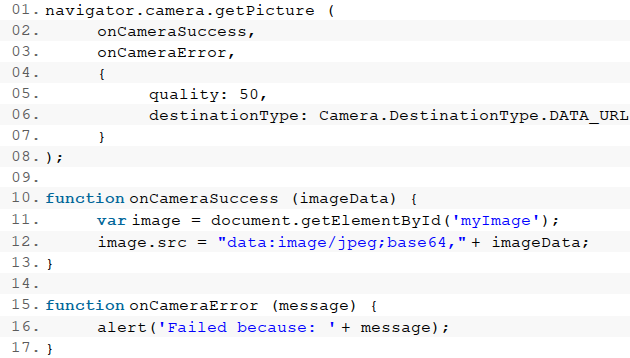
\includegraphics[scale=0.75]{Figures/exampleCordova.png} 
    \rule{35em}{0.5pt}
  \caption[Javascript API]{Un esempio di utilizzo di API Javascript per ottenere dati dalla fotocamera}
  \label{fig:Javascript API Example}
\end{figure}

Questa operazione non è possibile tramite un'implementazione come Web Application, perché per evidenti motivi di sicurezza, il Browser Web dei dispositivi mobili non ha libero accesso alle funzionalità del dispositivo(altrimenti qualunque sito internet potrebbe compromettere l'integrità dello stesso). Grazie a questo l'approccio ibrido si avvicina molto a quello nativo. Per fare questo le applicazioni ibride si servono di potenti framework che si occupano di fornire un canale di comunicazione tra le due entità, quella web e quella nativa, consentendo all'interfaccia scritta in HTML e Javascript di poter utilizzare le funzionalità del dispositivo. In particolare \emph{Cordova} è uno dei framewrok più usati per questo tipo di sviluppo, il quale fornisce dal lato dell'interfaccia web delle API in Javascript per comunicare con il dispositivo.

Sul mercato esistono framework che usano procedimenti differenti da quello appena spiegato per ottenere lo stesso risultato multi piattaforma, la maggior parte tende però a sviluppare l'interfaccia utente con codice
HTML, in quanto essendo un linguaggio tendenzialmente semplice consente di avere una descrizione dei dati accurata e dinamica molto rapidamente, la quale può essere riutilizzata se lo sviluppatore decidesse di avere una eventuale Web Application oltre a quella ibrida. Un punto molto forte dello sviluppo ibrido è appunto che è possibile riutilizzare il codice web, pur avendo una applicazione quasi nativa(ibrida).  

Prima del confronto tra gli approcci visti, verrà spiegato come i framework possono essere utili nello sviluppo di applicazioni mobili, e come possono risultare utili in particolare nell'approccio ibrido.

\section{Lo sviluppo di Applicazioni e i framework}
\label{sec:appAndFramework}
\textit{In informatica, e specificatamente nello sviluppo software, un \textbf{framework} è un'architettura (o più impropriamente struttura) logica di supporto (spesso un'implementazione logica di un particolare design pattern) su cui un software può essere progettato e realizzato, spesso facilitandone lo sviluppo da parte del programmatore. Alla base di un framework c'è sempre una serie di librerie di codice utilizzabili in fase di linking con uno o più linguaggi di programmazione, spesso corredate da una serie di strumenti di supporto allo sviluppo del software, come ad esempio un IDE, un debugger o altri strumenti ideati per aumentare la velocità di sviluppo del prodotto finito. L'utilizzo di un framework impone dunque al programmatore una precisa metodologia di sviluppo del software.}\\
\hspace*{\fill}\cite{wiki:framework}

L'uso di framework da parte di aziende e sviluppatori è diventato sempre più comune nello sviluppo di applicazioni mobile. Il processo di scrittura del codice diventa rapido e intuitivo, in alcuni casi si ha a disposizione un editor visuale dell'interfaccia che tramite il solo trascinamento di nuovi elementi, messi a disposizione dall'editor, aggiorna il codice sorgente dell'applicazione.
Oggi sul mercato esistono diversi tipi di framework, ognuno con caratteristiche e vantaggi differenti. Ciascuno di essi supporta uno o più sistemi operativi, ma non è detto che un framework possa supportare completamente le funzionalità richieste da un'applicazione e/o da un progetto.

Molti framework usano una combinazione di tecnologie, che ne caratterizza la loro tipologia, delle quali se ne distinguono 5: JavaScript framework, app factories, web-to-native wrapper, runtime e source code translator. A questo punto entrano in gioco le competenze del programmatore, il quale a seconda delle sue capacità sceglierà l'approccio più conveniente, in quanto per ognuno di essi sono coinvolte tecnologie differenti.
\cite{ref:bsc_waldner}

\begin{description}

\item[Javascript Framework] in alcuni casi sono semplicemente delle librerie e non propriamente dei framework e forniscono delle funzioni tipiche delle applicazioni mobile, come ad esempio, scorrimento e eventi legati al touch-screen. Principalemente si utilizzano per la costruzione della \emph{User Interface} i più conosciuti sono: JQuery Mobile, Ionic, Sencha Touch, Cocos2D, DHTMLX Touch, Zepto JS, Impact.js, iUI e Wink.

\item[App Factories] sono generatori di codice sorgente, ovvero sono dei tool grafici per costruire in modo semplice le applicazioni mobile. Sono composti di un ambiente di sviluppo (installabile o utilizzabile online) dove lo sviluppatore, partendo da un template base, inserisce elementi con il drag and drop, come ad esempio pulsanti ed input text. Infine le App factories generano il codice sorgente. App factories permettono ai non programmatori di “creare le loro app”. Alcuni tools permettono di vedere e modificare il codice generato. Altri includono una serie di servizi come analisi di utilizzo, push notification e gestionali.
Alcuni esempi di questi tool sono: AppMkr, AppsGeyser, Wix Mobile, Tiggr, Mobile Nation HQ, Mobjectify, Red Foundry e Spot Specific.

\item[Web-to-native Wrapper] questo tipo di framework fornisce un contenitore nativo all'interno del quale è possibile costruire una applicazione utilizzando tecnologie web. Il funzionamento è analogo come spiegato nella sezione \ref{sec:hybridApp}. Vengono estese le API di JavaScript e si ha la possibilità di accedere alle funzionalità del dispositivo e del sistema operativo come notifiche, accelerometro, bussola, geolocalizzazione e file system.
Il principale esempio di web-to-native wrapper è PhoneGap, ma ci sono anche Uxebu’s Apparat.io e Sencha v2 nella quale hanno aggiunto al wrapper dei framework JavaScript. Un altro esempio è MoSync Wormhole, il quale
dispone di un set di API come PhoneGap. Web-to-native wrapper mira agli sviluppatori web che hanno bisogno di convertire le loro applicazioni web ad applicazioni mobile per poterle pubblicare sui vari app store o anche per accedere alle funzionalità native del dispositivo e rendere il codice web ottimizzato nel contesto mobile.

\item[Runtime]è un approccio che, durante l'esecuzione di un applicazione, interpreta il codice sorgente da una virtual machine che è diversa a seconda del sistema operativo. Inoltre protegge l'applicazione dalle differenze tra le piattaforme sottostanti. Runtime varia in dimensione e complessità ed esegue codice sul dispositivo usando differenti metodi: la virtualizzazione, l'interpretazione, la compilazione just-in-time oppure la compilazione ahead-of-time. Java ME, BREW, Flash Lite e Openwave MIDAS sono stati i primi a sperimentare questo approccio sui dispositivi mobile. Queste virtual machine sono pesanti e sembrano una mezza via tra browser e sistema operativo. Oggigiorno questo tipo di approccio sposta la complessità delle operazioni dal software del dispositivo al design-time ovvero il momento di traduzione del codice in bytecode. Esempi di runtimes sono Appcelerator, Adobe Flex (e AIR), Corona, AppMobi, Antix e Unity.

\item[Source code translators]
Queste soluzioni traducono il codice sorgente in un bytecode intermedio, o in un linguaggio nativo (per esempio C++, Objective-C, JavaScript) o direttamente al linguaggio macchina di basso livello (linguaggio assembly). Source code translators sono spesso utilizzati in combinazione al runtime. Per esempio, Metismo (ora Software AG) converte applicazioni J2ME in C++, ActionScript e JavaScript, ed esse sono compilabili con dispositivi ARM, MIPS, PowerPC e x86. Analogamente, Eqela prende un applicazione scritta in un linguaggio simile al C e ne traduce il codice sorgente a seconda della piattaforma: JavaScript per web browsers, Java, C o assembly. 
\end{description}

Ecco una lista dei framework più conosciuti attualmente sul mercato:
\\
NOTA TESI: se si sceglie di inserire la tabella, differenziare i tipi di framework, e inserire l'url sotto forma di link nel nome del framework.
\\
\begin{table}[!htbp]
    \begin{tabular}{cc}
    \hline
    \textbf{NOME} 				 & \textbf{SITO WEB} 			                                \\\hline
    Appcelerator              	 & http://www.appcelerator.com/                                 \\\hline
    Corona                       & http://coronalabs.com                                        \\\hline
    Kony                         & http://www.kony.com                                          \\\hline
    PhoneGap                     & http://phonegap.com                                          \\\hline 
    Enyo                         & http://enyojs.com                                            \\\hline  
    eMobc                        & http://www.emobc.com                                         \\\hline
    iPFaces                      & http://www.ipfaces.org                                       \\\hline
    Sencha                       & http://www.sencha.com                                        \\\hline
    Steroids                     & http://www.appgyver.com/steroids                             \\\hline
    Trigger.io                   & https://trigger.io                                           \\\hline
    Intel App Framework          & http://app-framework-software.intel.com                      \\\hline
    Moai                         & http://getmoai.com                                           \\\hline
    Scirra / Construct 2         & https://www.scirra.com                                       \\\hline
    GameMaker Studio             & https://www.yoyogames.com/studio                             \\\hline
    Basic4android                & http://www.basic4ppc.com                                     \\\hline
    Kivy                         & http://kivy.org                                              \\\hline
    Syncfusion                   & http://www.syncfusion.com/solutions/mobility                 \\\hline
    Xamarin                      & https://xamarin.com                                          \\\hline
    Ionic                        & http://ionicframework.com/                                   \\\hline
    MoSync                       & http://www.mosync.com/                                       \\\hline
    GameSalad                    & http://gamesalad.com/                                        \\\hline
    Stencyl                      & http://www.stencyl.com/                                      \\\hline
    RAD Studio                   & http://www.embarcadero.com/products/rad-studio               \\\hline
    Telerik Mobile \\   
    Application Development\\
    Platform
    							 & http://www.telerik.com/platform                              \\\hline
    appery.io                    & http://appery.io                                             \\\hline
    RoboVM                       & http://www.robovm.org                                        \\\hline
    Marmalade                    & https://www.madewithmarmalade.com                            \\\hline
    CocoonJS                     & https://www.ludei.com/cocoonjs                               \\\hline
    Kendo UI Mobile              & http://www.telerik.com/kendo-ui-mobile                       \\\hline
    Microsoft XNA                & http://www.microsoft.com/en-us/download/details.aspx?id=20914\\\hline
    Unreal Engine                & http://www.unrealengine.com                                  \\\hline
    Ejecta                       & http://www.impactjs/comejecta                                \\\hline
    \end{tabular}
    \caption{Lista dei principali framework più conosciuti sul mercato}
	\label{tbl: TabellaFrameworks}
\end{table}



\section{Conclusioni}

Nel confronto tra lo sviluppo nativo e quello tramite Web Application si è visto che i principali fattori a pesare su un obiettivo di applicazione multi piattaforma è la possibilità di accedere alle funzionalità del dispositivo e di avere prestazioni molto efficienti contro una portabilità immediata senza il bisogno di riscrivere il codice per ogni piattaforma di destinazione. 
Introducendo le applicazioni ibride si è potuto combinare entrambi i fattori positivi dei due approcci differenti, infatti in questo tipo di approccio si può accedere alle funzionalità del dispositivo tramite delle API che un framework di supporto fornisce, ma riguardo alle prestazioni, non si è ancora arrivati ad una tecnologia che consenta di paragonare l'efficienza dello sviluppo nativo con quello di tipo ibrido. Con l'evoluzione delle tecnologie utilizzate dai framework e il continuo susseguirsi versioni di piattaforme sempre più adattabili a diversi tipi di tecnologie, il distacco tra i due approcci continua sempre a diminuire.

\subsection{Qual'è l'approccio migliore}

Non esiste un approccio migliore di un altro in quanto hanno tutti pregi e difetti sotto certi punti di vista, in base allo scopo e ai requisiti dell'applicazione che si vuole creare bisogna valutare quale approccio sia il migliore da utilizzare per poter competere al meglio sul mercato.
Un esempio potrebbe essere una applicazione gioco, la quale richiede una forte potenza di calcolo a livello grafico e che con uno sviluppo di tipo ibrido o web è molto difficile da ottenere. In questi casi quando le prestazioni sono al centro della richiesta dell'applicazione, uno sviluppo di tipo nativo, anche se più dispendioso in quanto si resta sotto l'idea di avere una applicazione multi piattaforma, è una delle scelte migliori che si possono fare.
Una alternativa potrebbe ese.
sere quella di utilizzare un framework apposito allo sviluppo di giochi, che consenta di avere un gioco multi piattaforma, si ricorda però che alcuni tipi di framework molto avanzati spesso non sono open source e richiedono un investimento da parte del programmatore / azienda per il suo utilizzo.
Nel caso l'applicazione richieda una potenza di calcolo nella media la scelta dell'approccio e delle tecnologie da utilizzare ricade sulle caratteristiche specifiche che l'applicazione richiede.


\subsection{L'importanza della scelta del framework}

Oggi sul mercato esistono diversi tipi di framework, ognuno con caratteristiche e vantaggi differenti. Ciascuno di essi supporta uno o più sistemi operativi, ma non è detto che un framework possa supportare completamente le funzionalità richieste da un'applicazione e da un progetto.
Per questo motivo la scelta del framework giusto deve essere oggetto di una attenta valutazione da parte delle aziende o dei programmatori. Questa valutazione deve prendere in considerazione numerosi parametri quali, ad esempio, le funzionalità che il cliente intende integrare nell'applicazione, i dispositivi sui quali questa applicazione deve girare, il budget a disposizione, il termine ultimo per commercializzare l'applicazione sul mercato ed infine la strategia di lungo termine legata alla quantità di progetti che devono essere sviluppati.
Tutti i framework, come sopra accennato, non supportano tutti i sistemi operativi. Per questo motivo l'esperienza del programmatore è fondamentale per ottimizzare gli strumenti di sviluppo e le funzionalità dell'applicazione.

Il vantaggio principale nell'utilizzo di un framework consiste nella possibilità di effettuare una consegna rapida e multi piattaforma di un'applicazione: il codice, infatti, si scrive velocemente con un meta linguaggio ed attraverso librerie esistenti precompilate, ed esso viene automaticamente adattato per i diversi sistemi operativi in fase di compilazione.

Una criticità di questo tipo di framework consiste nel fatto che, all'inizio, l'azienda deve sostenere costi piuttosto elevati per l'acquisto della licenza. Occorre inoltre investire anche nelle attività di formazione per le risorse interne che dovranno occuparsi dell'implementazione e dell'uso del framework. Un limite ulteriore dei framework consiste nell'eccesso di rigidità in fase progettuale: il loro utilizzo, infatti, limita in parte la possibilità di sfruttare le caratteristiche native del dispositivo, delle linee guida dell'interfaccia e del sistema operativo che utilizzerà l'applicazione, e spesso, quindi, si corre il rischio di non riuscire a sviluppare interfacce utente pienamente ergonomiche e intuitive.

Nella scelta del framework occorre anche concentrarsi su quelli che offrono una maggiore garanzia di supporto nel corso del tempo. Alcuni framework infatti tendono a non essere più supportati dopo un certo periodo di tempo; in questo caso, se occorre implementare sviluppi ulteriori, si corre il rischio di dover riprogettare l'applicazione da zero utilizzando un framework diverso.

Inoltre, alcuni framework sono più adatti ad impieghi specifici rispetto ad altri. Kony, ad esempio, è un tipo di framework particolarmente apprezzato nello sviluppo di applicazioni per il settore bancario e financial, poichè integra al suo interno numerose funzioni utili, ad esempio, per la gestione dei sistemi di pagamento attraverso gli smartphone. Unity 3D, invece, è il framework ideale per lo sviluppo di giochi e videogames.

Nel caso di framework nativi i costi iniziali sono più bassi rispetto ai precedenti (non vi è, ad esempio, la necessità di acquistare la licenza per il loro utilizzo), tuttavia i costi tendono a crescere esponenzialmente in funzione della quantità di aggiornamenti e rilasci da effettuare nel corso del tempo, o  nel caso in cui si intenda sviluppare un’applicazione per più sistemi operativi diversi tra loro.

Un tipo di framework scelto nel contesto giusto, che tenga concretamente conto degli obiettivi di marketing dell'azienda e le strategie di investimento in sviluppo di prodotti, consente di ottimizzare i tempi di sviluppo, presentare velocemente sul mercato la propria applicazione ed ottimizzare il processo di delivery abbattendo costi e sfruttando le potenzialità specifiche del framework selezionato.

\subsection{E' possibile uno sviluppo multi piattaforma senza l'utilizzo di framework?}

Si è inteso lo sviluppo multi piattaforma come partendo da un unico codice sorgente dell'applicazione ad avere quest'ultima già disponibile per più di un canale di distribuzione sul mercato(ovvero i sistemi operativi dei dispositivi, la web application). Ebbene questo procedimento senza un framework di supporto risulta molto difficoltoso in quanto l'approccio rimane quello nativo per ogni piattaforma, oppure il programmatore / azienda ha a disposizione un sistema proprietario progettato appositamente per fare questa operazione, opzione che non è mai presa in considerazione in quanto molto dispendiosa.
Per uno sviluppo multi piattaforma è richiesta la conoscenza del funzionamento di almeno un framework, che dipende sostanzialmente dalle conoscenze e dalla formazione del programmatore, il quale sceglierà le tecnologie più adatte alle sue conoscenze pregresse.
  


   







